\documentclass[aspectratio=169, 10pt]{beamer}

% ---------- Tema y colores ----------
\usetheme{default}
\usecolortheme{default}
\setbeamertemplate{navigation symbols}{}
\setbeamertemplate{footline}[frame number]
\setbeamertemplate{frametitle continuation}{}

\definecolor{StanfordRed}{RGB}{140,21,21}
\definecolor{StanfordGray}{RGB}{77,77,77}
\definecolor{LightGray}{RGB}{240,240,240}
\definecolor{AccentBlue}{RGB}{0,84,166}
\definecolor{AccentGreen}{RGB}{0,130,100}
\definecolor{UCMBlue}{RGB}{4, 171, 226}
\definecolor{UCMNavy}{RGB}{20, 65, 134}

% Alias de la paleta antigua: las figuras TikZ de esta clase siguen
% usando mitblue/mitgray, que ahora apuntan a los colores UCM.
\definecolor{mitblue}{RGB}{20, 65, 134}
\definecolor{mitgray}{RGB}{169, 169, 169}

\setbeamercolor{frametitle}{fg=white, bg=UCMBlue}
\setbeamercolor{title}{fg=white}
\setbeamercolor{author}{fg=white}
\setbeamercolor{institute}{fg=white!80}
\setbeamercolor{structure}{fg=UCMBlue}
\setbeamercolor{block title}{bg=UCMBlue!15!white, fg=UCMBlue}
\setbeamercolor{block body}{bg=LightGray}
\setbeamercolor{block title alerted}{bg=StanfordRed!15!white, fg=StanfordRed}
\setbeamercolor{block body alerted}{bg=LightGray}
\setbeamercolor{block title example}{bg=AccentGreen!15!white, fg=AccentGreen}
\setbeamercolor{block body example}{bg=LightGray}
\setbeamercolor{alerted text}{fg=UCMBlue}
\setbeamercolor{example text}{fg=UCMBlue}

\setbeamerfont{frametitle}{series=\bfseries, size=\large}
\setbeamerfont{title}{series=\bfseries, size=\LARGE}
\setbeamerfont{block title}{series=\bfseries}

% ---------- Paquetes ----------
\usepackage[utf8]{inputenc}
\usepackage[T1]{fontenc}
\usepackage[provide=*,spanish]{babel}
\usepackage{amsmath, amssymb, bm}
\usepackage{graphicx}
\usepackage{tikz}
\usepackage{pgfplots}
\pgfplotsset{compat=1.18}
\usetikzlibrary{arrows, arrows.meta, shapes, shapes.geometric, positioning,
	fit, calc, matrix, chains, mindmap, decorations.pathreplacing,
	backgrounds, shadows, patterns}
\usepackage{booktabs}
\usepackage{xcolor}
\usepackage{multicol}
\usepackage{tcolorbox}
\tcbuselibrary{skins, breakable}
\usepackage{ragged2e}


% ---------- Comandos útiles ----------
\providecommand{\R}{\mathbb{R}}
\providecommand{\E}{\mathbb{E}}
\providecommand{\Var}{\operatorname{Var}}
\providecommand{\relu}{\operatorname{ReLU}}
\providecommand{\Pa}{\operatorname{Pa}}
% Independencia condicional
\newcommand{\indep}{\perp\!\!\!\perp}
\newcommand{\nindep}{\not\!\perp\!\!\!\perp}

\newcommand{\formula}[1]{%
	\begin{tcolorbox}[colback=UCMBlue!8, colframe=UCMBlue, arc=4pt,
		boxsep=2pt, left=6pt, right=6pt, top=3pt, bottom=3pt]
		#1
	\end{tcolorbox}
}

% Caja para una idea clave / lectura de un diagrama
\newcommand{\idea}[1]{%
	\begin{tcolorbox}[colback=AccentGreen!6, colframe=AccentGreen, arc=3pt,
		width=\textwidth, boxsep=1pt, left=5pt, right=5pt, top=2pt, bottom=2pt,
		fontupper=\small]
		\RaggedRight\textbf{Idea clave:} #1
	\end{tcolorbox}
}

% Caja para una regla de producción SI...ENTONCES
\newcommand{\regla}[2]{%
	\begin{tcolorbox}[colback=LightGray, colframe=UCMNavy, arc=3pt,
		boxsep=1pt, left=5pt, right=5pt, top=2pt, bottom=2pt,
		fontupper=\small, title={\scriptsize\bfseries #1},
		fonttitle=\scriptsize\bfseries, coltitle=white, colbacktitle=UCMNavy]
		\RaggedRight #2
	\end{tcolorbox}
}

% ---------- Portada ----------
\title{\textbf{Sistemas Expertos}}
\subtitle{El paradigma simb\'olico de la IA}
\author{Sergio Hern\'andez, PhD\\ shernandez@ucm.cl}
\institute{
	\begin{tikzpicture}[scale=0.42, every node/.style={transform shape}]
		\foreach \i/\y in {1/0,2/1,3/2}{\node[circle,draw=white,fill=white!20,minimum size=4mm] (i\i) at (0,\y){};}
		\foreach \i/\y in {1/-0.5,2/0.5,3/1.5,4/2.5}{\node[circle,draw=white,fill=white!35,minimum size=4mm] (h\i) at (2,\y){};}
		\foreach \i/\y in {1/0.5,2/1.5}{\node[circle,draw=white,fill=white!50,minimum size=4mm] (o\i) at (4,\y){};}
		\foreach \a in {1,2,3}\foreach \b in {1,2,3,4}{\draw[white,opacity=0.5] (i\a)--(h\b);}
		\foreach \a in {1,2,3,4}\foreach \b in {1,2}{\draw[white,opacity=0.5] (h\a)--(o\b);}
	\end{tikzpicture}
	\\ \textbf{Mag\'ister en Data Science --- Universidad Cat\'olica del Maule}}
\date{}


\begin{document}
% --- Título ---
{
	\setbeamertemplate{background}{
		\begin{tikzpicture}[remember picture, overlay]
			\fill[UCMBlue] (current page.south west) rectangle (current page.north east);
			\fill[UCMBlue!70!black, opacity=0.5]
			(current page.south west) -- ++(0,3) -- ++(18,0) -- cycle;
			\foreach \i in {1,...,40}{
				\fill[white, opacity=0.04]
				({random()*17}, {random()*10}) circle ({random()*0.3});
			}
		\end{tikzpicture}
	}
	\begin{frame}[plain]
		\vspace{1.2cm}
		\titlepage
		\begin{tikzpicture}[remember picture, overlay]
			\node[white, opacity=0.15, font=\fontsize{80}{80}\selectfont]
			at (current page.east) [xshift=-2cm] {$\Rightarrow$};
		\end{tikzpicture}
	\end{frame}
}

\begin{frame}
\frametitle{Hoja de ruta}
\begin{columns}[T]
\begin{column}{6cm}
\begin{enumerate}
	\item ¿Qué es un sistema experto?
	\item Representar el conocimiento: l\'ogica proposicional
	\item Inferir: el motor de reglas
\end{enumerate}
\end{column}
\begin{column}{6cm}
\begin{enumerate}
	\setcounter{enumi}{3}
	\item Incertidumbre: modelos gr\'aficos probabil\'isticos
	\item Historia, l\'imites y legado
	\item Cierre y lecturas
\end{enumerate}
\end{column}
\end{columns}
\vspace{0.8em}
\begin{block}{Objetivo de la clase}
Entender el \textbf{paradigma simb\'olico} en concreto: c\'omo se escribe una base de conocimiento, c\'omo un motor de inferencia encadena reglas, y por qu\'e este enfoque triunf\'o y despu\'es se estanc\'o. Al final, la respuesta formal a su punto d\'ebil: representar el conocimiento incierto con una \textbf{red bayesiana}.
\end{block}
\end{frame}

%=====================================================================
\section{¿Qué es un sistema experto?}
%=====================================================================

\begin{frame}
\frametitle{IA simbólica: la promesa}
\begin{block}{Sistemas expertos}
Programas que resuelven problemas de un \textbf{dominio acotado} emulando el razonamiento de un especialista humano, a partir de conocimiento \textbf{declarado explícitamente} y no aprendido de los datos.
\end{block}
\pause
\begin{columns}[T]
\begin{column}{6cm}
\begin{itemize}
	\item Fueron el primer \'exito \textbf{comercial} de la IA (d\'ecada de 1980).
	\item El conocimiento se escribe, se lee y se audita: cada conclusi\'on tiene una traza.
\end{itemize}
\end{column}
\begin{column}{6cm}
\begin{itemize}
	\item Contraste con la clase anterior: aqu\'i el programador \textbf{escribe la regla}; en aprendizaje autom\'atico escribe el \textbf{objetivo} y la regla se ajusta sola.
	\item Ambos enfoques conviven hoy en sistemas h\'ibridos.
\end{itemize}
\end{column}
\end{columns}
\end{frame}

\begin{frame}
\frametitle{Del dato a la decisión}
\begin{columns}[c]
\begin{column}{6.0cm}
\begin{center}
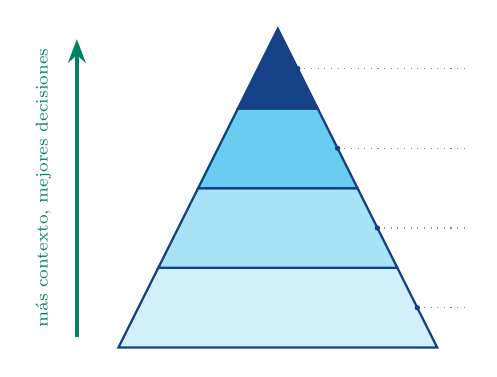
\begin{tikzpicture}[scale=0.88, transform shape]
	% bandas de la pirámide: y va de 0 a 4.6, semiancho 2.3*(1-y/4.6)
	\foreach \i/\col in {0/UCMBlue!18, 1/UCMBlue!35, 2/UCMBlue!60, 3/UCMNavy}{
		\fill[\col, draw=UCMNavy, thick]
			({-2.3*(1-\i/4)}, {\i*1.15}) --
			({ 2.3*(1-\i/4)}, {\i*1.15}) --
			({ 2.3*(1-(\i+1)/4)}, {(\i+1)*1.15}) --
			({-2.3*(1-(\i+1)/4)}, {(\i+1)*1.15}) -- cycle;
	}
	% conectores hacia las etiquetas de la derecha
	\foreach \i in {0,1,2,3}{
		\draw[UCMNavy!60, dotted] ({2.3*(1-(\i+0.5)/4)}, {(\i+0.5)*1.15}) -- (2.75, {(\i+0.5)*1.15});
		\fill[UCMNavy] ({2.3*(1-(\i+0.5)/4)}, {(\i+0.5)*1.15}) circle (1.1pt);
	}
	% flecha de progresión
	\draw[-{Stealth[length=3mm]}, very thick, AccentGreen] (-2.9,0.15) -- (-2.9,4.45);
	\node[AccentGreen, font=\scriptsize, rotate=90, anchor=south] at (-3.15,2.3) {m\'as contexto, mejores decisiones};
\end{tikzpicture}
\end{center}
\end{column}
\begin{column}{6.2cm}
\footnotesize
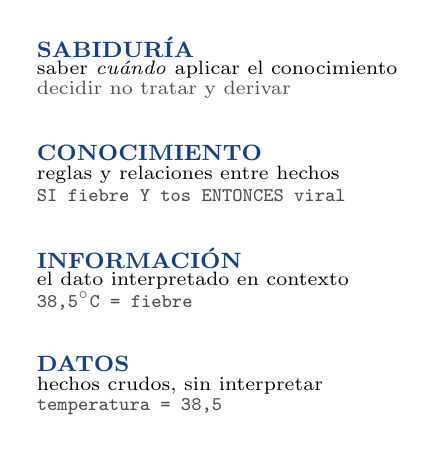
\begin{tikzpicture}[font=\footnotesize]
	\foreach \i/\lab/\desc/\ej in {
		3/SABIDUR\'IA/{saber \emph{cu\'ando} aplicar el conocimiento}/{decidir no tratar y derivar},
		2/CONOCIMIENTO/{reglas y relaciones entre hechos}/{\texttt{SI fiebre Y tos ENTONCES viral}},
		1/INFORMACI\'ON/{el dato interpretado en contexto}/{\texttt{38{,}5$^\circ$C = fiebre}},
		0/DATOS/{hechos crudos, sin interpretar}/{\texttt{temperatura = 38{,}5}}}{
		\node[anchor=west, font=\bfseries\footnotesize, text=UCMNavy] at (0, {\i*1.34+0.28}) {\lab};
		\node[anchor=west, font=\scriptsize] at (0, {\i*1.34}) {\desc};
		\node[anchor=west, font=\scriptsize, text=StanfordGray] at (0, {\i*1.34-0.26}) {\ej};
	}
\end{tikzpicture}
\end{column}
\end{columns}
\vspace{0.2em}
\idea{Un sistema experto vive en el tercer nivel: su valor no est\'a en almacenar datos, sino en codificar las \textbf{reglas} que un especialista aplica sobre ellos.}
\end{frame}

\begin{frame}
\frametitle{Anatomía de un sistema experto}
\begin{center}
\scalebox{0.87}{%
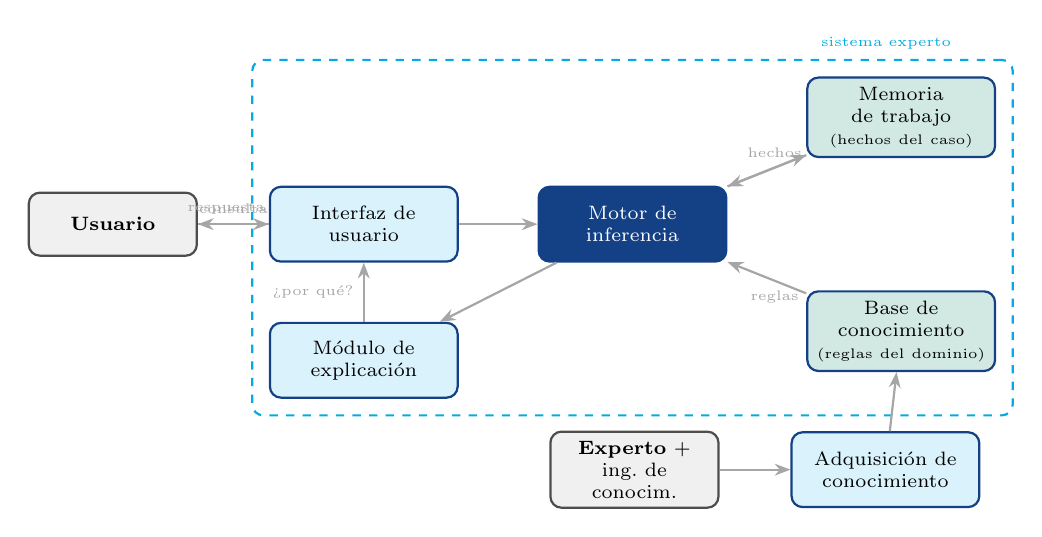
\begin{tikzpicture}[font=\scriptsize, node distance=0.6cm,
	caja/.style={rectangle, draw=UCMNavy, thick, rounded corners, align=center,
		text width=2.15cm, minimum height=0.95cm, fill=UCMBlue!15},
	nucleo/.style={caja, fill=UCMNavy, text=white},
	dato/.style={caja, fill=AccentGreen!18},
	persona/.style={rectangle, draw=StanfordGray, thick, rounded corners, align=center,
		text width=1.9cm, minimum height=0.8cm, fill=LightGray},
	fl/.style={-{Stealth[length=2mm]}, thick, gray!70}]

	\node[persona] (user) at (0,0) {\textbf{Usuario}};
	\node[caja, right=0.9cm of user] (ui) {Interfaz de usuario};
	\node[nucleo, right=1.0cm of ui] (motor) {Motor de\\inferencia};
	\node[dato, above right=0.35cm and 1.0cm of motor] (mem) {Memoria de trabajo\\{\tiny(hechos del caso)}};
	\node[dato, below right=0.35cm and 1.0cm of motor] (bc) {Base de conocimiento\\{\tiny(reglas del dominio)}};
	\node[caja, below=0.75cm of ui] (expl) {M\'odulo de explicaci\'on};
	\node[caja, below=0.75cm of bc, xshift=-0.2cm] (adq) {Adquisici\'on de conocimiento};
	\node[persona, left=0.9cm of adq] (exp) {\textbf{Experto} +\\ing.\ de conocim.};

	\draw[fl] (user) -- node[above, font=\tiny] {consulta} (ui);
	\draw[fl] (ui) -- (motor);
	\draw[fl] (motor) -- (mem);
	\draw[fl] (mem) -- node[above, font=\tiny, pos=0.4] {hechos} (motor);
	\draw[fl] (bc) -- node[below, font=\tiny, pos=0.4] {reglas} (motor);
	\draw[fl] (motor) -- (expl);
	\draw[fl] (expl) -- node[left, font=\tiny] {¿por qu\'e?} (ui);
	\draw[fl] (ui) -- node[above, font=\tiny, pos=0.6] {respuesta} (user);
	\draw[fl] (exp) -- (adq);
	\draw[fl] (adq) -- (bc);

	\begin{scope}[on background layer]
		\node[draw=UCMBlue, dashed, thick, rounded corners, inner sep=6pt,
			fit=(ui)(motor)(mem)(bc)(expl), label={[font=\tiny, text=UCMBlue]above right:sistema experto}] {};
	\end{scope}
\end{tikzpicture}}
\end{center}
\vspace{0.2em}
\idea{La separaci\'on entre \textbf{conocimiento} (las reglas, que cambian) y \textbf{control} (el motor, que no cambia) es lo que permite reutilizar un mismo motor en dominios distintos: es la arquitectura de un \emph{shell}.}
\end{frame}

\begin{frame}
\frametitle{Cuatro características que los definen}
\begin{columns}[T]
\begin{column}{6cm}
\begin{block}{Heurísticos}
Codifican \emph{reglas de buena pr\'actica} del especialista, no un modelo matem\'atico cerrado del dominio.
\end{block}
\begin{block}{Explicables}
Pueden reconstruir la cadena de reglas que llev\'o a la conclusi\'on. Hoy lo llamamos \textbf{XAI}.
\end{block}
\end{column}
\begin{column}{6cm}
\begin{block}{Conocimiento separado del control}
La base de reglas se edita sin tocar el motor. Permite que el \emph{experto} colabore sin programar.
\end{block}
\begin{block}{Toleran incertidumbre}
Trabajan con informaci\'on incompleta mediante \textbf{factores de certeza} o probabilidades.
\end{block}
\end{column}
\end{columns}
\vspace{0.5em}
\footnotesize A cambio, el dominio debe ser \textbf{estrecho y estable}: nada de sentido com\'un ni de conocimiento general.
\end{frame}

%=====================================================================
\section{Representar el conocimiento: lógica proposicional}
%=====================================================================

\begin{frame}
\frametitle{Proposiciones y conectivas}
\begin{columns}[T]
\begin{column}{6.6cm}
\begin{itemize}
	\item Una \textbf{proposici\'on} es un enunciado sobre el mundo que solo puede ser verdadero o falso.
	\item Se abrevian con s\'imbolos: $P$, $Q$, $R$.
	\item Las \textbf{conectivas} combinan proposiciones para expresar afirmaciones compuestas.
\end{itemize}
\vspace{0.3em}
\footnotesize
\textbf{Ejemplo del dominio m\'edico:}\\
$P$: \emph{el paciente tiene fiebre}\qquad $Q$: \emph{el paciente tiene tos seca}\\
$P \land Q \rightarrow R$: \emph{si tiene fiebre y tos seca, hay infecci\'on viral}.
\end{column}
\begin{column}{5.4cm}
\begin{center}
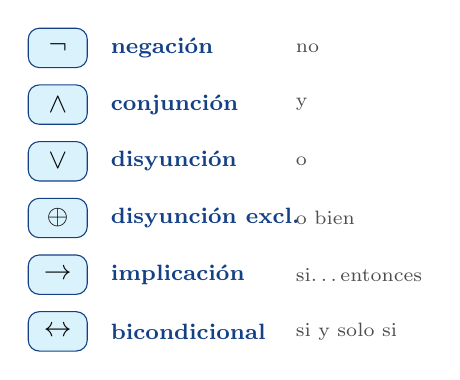
\begin{tikzpicture}[font=\small, every node/.style={anchor=west}]
	\foreach \s/\n/\l [count=\i from 0] in {
		{$\neg$}/negaci\'on/{no},
		{$\land$}/conjunci\'on/{y},
		{$\lor$}/disyunci\'on/{o},
		{$\oplus$}/disyunci\'on excl./{o bien},
		{$\rightarrow$}/implicaci\'on/{si\ldots entonces},
		{$\leftrightarrow$}/bicondicional/{si y solo si}}{
		\node[fill=UCMBlue!15, draw=UCMNavy, rounded corners, minimum width=0.75cm,
			minimum height=0.5cm, anchor=center, font=\normalsize] at (0,-0.72*\i) {\s};
		\node[font=\footnotesize\bfseries, text=UCMNavy] at (0.55,-0.72*\i) {\n};
		\node[font=\scriptsize, text=StanfordGray] at (2.9,-0.72*\i) {\l};
	}
\end{tikzpicture}
\end{center}
\end{column}
\end{columns}
\end{frame}

\begin{frame}
\frametitle{Las seis conectivas en una sola tabla}
\begin{center}
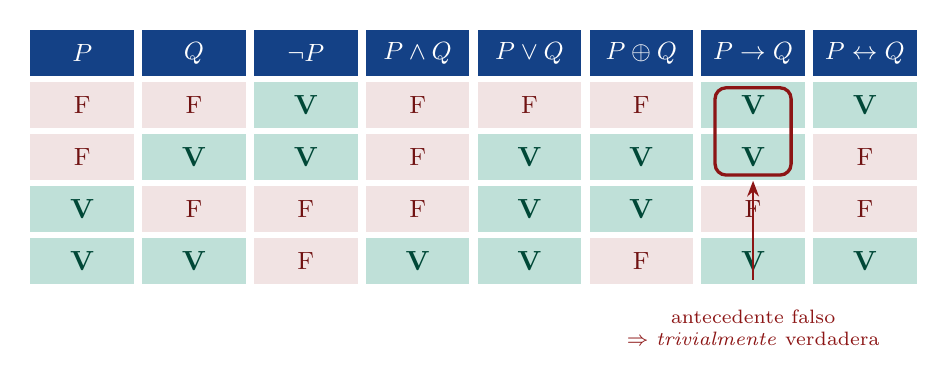
\begin{tikzpicture}[x=1.42cm, y=0.66cm, font=\small,
	celda/.style={minimum width=1.35cm, minimum height=0.62cm, anchor=center,
		draw=white, line width=1pt},
	V/.style={celda, fill=AccentGreen!25, text=AccentGreen!55!black, font=\bfseries},
	F/.style={celda, fill=StanfordRed!12, text=StanfordRed!80!black},
	cab/.style={celda, fill=UCMNavy, text=white, font=\small\bfseries}]

	\foreach \t [count=\c from 0] in {$P$, $Q$, $\neg P$, $P\land Q$, $P\lor Q$,
		$P\oplus Q$, $P\rightarrow Q$, $P\leftrightarrow Q$}{
		\node[cab] at (\c,0) {\t};
	}
	\foreach \r/\vals in {1/{F,F,V,F,F,F,V,V},
	                      2/{F,V,V,F,V,V,V,F},
	                      3/{V,F,F,F,V,V,F,F},
	                      4/{V,V,F,V,V,F,V,V}}{
		\foreach \v [count=\c from 0] in \vals{
			\node[\v] at (\c,-\r) {\v};
		}
	}
	% las dos entradas contraintuitivas de la implicación
	\draw[StanfordRed, very thick, rounded corners]
		(5.66,-0.66) rectangle (6.34,-2.34);
	\node[StanfordRed, font=\scriptsize, anchor=north, align=center] at (6,-4.75)
		{antecedente falso\\$\Rightarrow$ \emph{trivialmente} verdadera};
	\draw[StanfordRed, thick, -{Stealth[length=2mm]}] (6,-4.35) -- (6,-2.45);
\end{tikzpicture}
\end{center}
\vspace{0.1em}
\idea{$P \rightarrow Q$ \textbf{no} afirma causalidad: solo excluye el caso $P$ verdadero con $Q$ falso. \emph{Si la luna es de queso, apruebo el ramo} es una proposici\'on verdadera.}
\end{frame}

\begin{frame}
\frametitle{Base de conocimiento y modelos}
\begin{columns}[T]
\begin{column}{6.4cm}
\begin{itemize}
	\item Una \textbf{base de conocimiento} (KB) es el conjunto de sentencias que el agente da por ciertas.
	\item Un \textbf{modelo} es una asignaci\'on de verdadero/falso a \emph{todas} las proposiciones: una forma posible del mundo.
	\item Con $n$ proposiciones hay $2^{n}$ modelos.
\end{itemize}
\vspace{0.3em}
\formula{\centering KB $\models \alpha$ \; si $\alpha$ es verdadera en \emph{todo} modelo donde KB lo es.}
\end{column}
\begin{column}{5.6cm}
\begin{center}
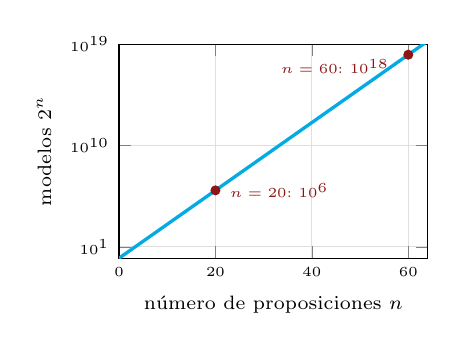
\begin{tikzpicture}
\begin{axis}[width=5.5cm, height=4.3cm, ymode=log,
	xlabel={n\'umero de proposiciones $n$}, ylabel={modelos $2^n$},
	xlabel style={font=\scriptsize}, ylabel style={font=\scriptsize},
	tick label style={font=\tiny}, grid=major, grid style={gray!25},
	xmin=0, xmax=64, ymin=1, ymax=1e19]
	\addplot[UCMBlue, very thick, domain=0:64, samples=40]{2^x};
	\addplot[only marks, mark=*, StanfordRed, mark size=1.6pt]
		coordinates {(20,1048576) (60,1.15e18)};
	\node[font=\tiny, StanfordRed, anchor=west] at (axis cs:21,1e6) {$n=20$: $10^6$};
	\node[font=\tiny, StanfordRed, anchor=east] at (axis cs:58,1e17) {$n=60$: $10^{18}$};
\end{axis}
\end{tikzpicture}
\end{center}
\end{column}
\end{columns}
\vspace{0.2em}
\idea{Comprobar la consecuencia enumerando modelos (\emph{model checking}) es correcto pero inviable: por eso los sistemas expertos no enumeran mundos, sino que \textbf{aplican reglas}.}
\end{frame}

\begin{frame}
\frametitle{Implicación ($\rightarrow$) vs. consecuencia lógica ($\models$)}
\begin{columns}[T]
\begin{column}{6cm}
\begin{itemize}
	\item $\rightarrow$ es una \textbf{conectiva}: construye una nueva proposici\'on, que puede ser verdadera o falsa.
	\item $\models$ es una \textbf{relaci\'on} entre conjuntos de sentencias: se cumple o no se cumple, y se verifica sobre \emph{todos} los modelos.
\end{itemize}
\vspace{0.3em}
\footnotesize
Si $\alpha$: \emph{es martes de enero} y $\beta$: \emph{es enero}, entonces $\alpha \models \beta$: no existe ning\'un mundo donde lo primero valga y lo segundo no.
\end{column}
\begin{column}{6cm}
\begin{center}
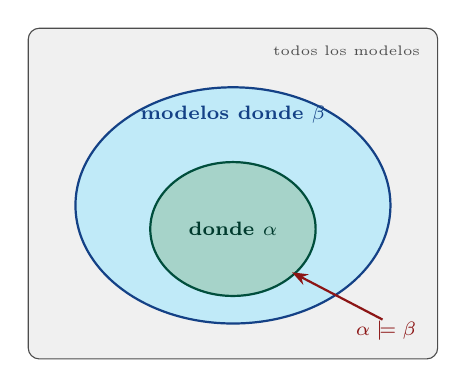
\begin{tikzpicture}[font=\scriptsize]
	\draw[draw=StanfordGray, fill=LightGray, rounded corners] (-2.6,-2.1) rectangle (2.6,2.1);
	\node[anchor=north east, font=\tiny, text=StanfordGray] at (2.5,2.0) {todos los modelos};
	\fill[UCMBlue!25, draw=UCMNavy, thick] (0,-0.15) ellipse (2.0 and 1.5);
	\fill[AccentGreen!35, draw=AccentGreen!60!black, thick] (0,-0.45) ellipse (1.05 and 0.85);
	\node[text=UCMNavy, font=\scriptsize\bfseries] at (0,1.0) {modelos donde $\beta$};
	\node[font=\scriptsize\bfseries, text=AccentGreen!45!black] at (0,-0.45) {donde $\alpha$};
	\draw[-{Stealth[length=2mm]}, thick, StanfordRed] (1.9,-1.6) -- (0.75,-1.0);
	\node[anchor=north east, font=\scriptsize, text=StanfordRed] at (2.45,-1.5)
		{$\alpha \models \beta$};
\end{tikzpicture}
\end{center}
\end{column}
\end{columns}
\vspace{0.2em}
\idea{$\alpha \models \beta$ significa que el conjunto de mundos donde $\alpha$ es verdadera est\'a \textbf{contenido} en aquel donde $\beta$ lo es.}
\end{frame}

%=====================================================================
\section{Inferencia: el motor de reglas}
%=====================================================================

\begin{frame}
\frametitle{La regla que ejecuta el motor: \emph{modus ponens}}
\begin{columns}[T]
\begin{column}{5.6cm}
\begin{center}
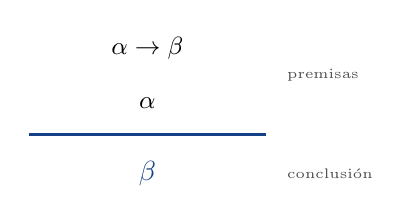
\begin{tikzpicture}[font=\small]
	\node (a) at (0,0.85) {$\alpha \rightarrow \beta$};
	\node (b) at (0,0.15) {$\alpha$};
	\draw[very thick, UCMNavy] (-1.5,-0.25) -- (1.5,-0.25);
	\node[text=UCMNavy, font=\bfseries] (c) at (0,-0.75) {$\beta$};
	\node[anchor=west, font=\tiny, text=StanfordGray] at (1.65,0.5) {premisas};
	\node[anchor=west, font=\tiny, text=StanfordGray] at (1.65,-0.75) {conclusi\'on};
\end{tikzpicture}
\end{center}
\vspace{0.4em}
\footnotesize
Si sabemos que \emph{si llueve, Harry est\'a dentro} y adem\'as \emph{llueve}, podemos afirmar \emph{Harry est\'a dentro}.
\end{column}
\begin{column}{6.4cm}
\begin{block}{Otras reglas de inferencia útiles}
\footnotesize
\begin{tabular}{@{}ll@{}}
\toprule
\textbf{Regla} & \textbf{De\ldots\ se deduce} \\
\midrule
Eliminaci\'on de $\land$    & $\alpha \land \beta \;\Rightarrow\; \alpha$ \\
Doble negaci\'on            & $\neg(\neg\alpha) \;\Rightarrow\; \alpha$ \\
Eliminaci\'on de $\rightarrow$ & $\alpha \rightarrow \beta \;\Rightarrow\; \neg\alpha \lor \beta$ \\
De Morgan                   & $\neg(\alpha \land \beta) \;\Rightarrow\; \neg\alpha \lor \neg\beta$ \\
Resoluci\'on                & $\alpha\lor\beta,\;\neg\beta\lor\gamma \;\Rightarrow\; \alpha\lor\gamma$ \\
\bottomrule
\end{tabular}
\end{block}
\end{column}
\end{columns}
\vspace{0.2em}
\idea{Aplicar reglas de inferencia genera conclusiones \textbf{sin enumerar los $2^n$ modelos}. Es la diferencia entre demostrar y verificar por fuerza bruta.}
\end{frame}

\begin{frame}
\frametitle{Del cálculo a la práctica: reglas de producción}
En un sistema experto el conocimiento no se escribe como f\'ormulas sueltas, sino como \textbf{reglas de producci\'on} sobre una memoria de hechos:
\vspace{0.3em}
\begin{columns}[T]
\begin{column}{6.2cm}
\regla{R1}{\textbf{SI} fiebre \textbf{Y} tos seca\\ \textbf{ENTONCES} infecci\'on viral}
\regla{R2}{\textbf{SI} infecci\'on viral \textbf{Y} dolor muscular\\ \textbf{ENTONCES} gripe}
\end{column}
\begin{column}{6.2cm}
\regla{R3}{\textbf{SI} fiebre \textbf{Y} manchas cut\'aneas\\ \textbf{ENTONCES} infecci\'on bacteriana}
\vspace{0.2em}
\footnotesize
\textbf{Hechos observados en el caso:}\\
\texttt{fiebre}, \texttt{tos seca}, \texttt{dolor muscular}.
\end{column}
\end{columns}
\vspace{0.4em}
\begin{itemize}
	\item Cada regla es \emph{modus ponens} disfrazado: antecedente $\rightarrow$ consecuente.
	\item El motor decide \textbf{en qu\'e orden} probarlas. Hay dos estrategias, y esa elecci\'on lo cambia todo.
\end{itemize}
\end{frame}

\begin{frame}
\frametitle{Encadenamiento hacia adelante (\emph{forward chaining})}
\begin{center}
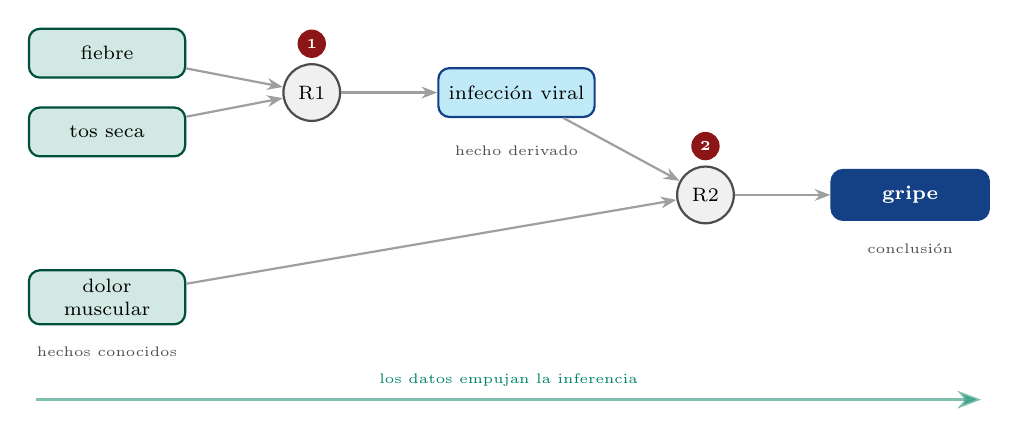
\begin{tikzpicture}[font=\scriptsize,
	hecho/.style={rectangle, draw=AccentGreen!60!black, thick, rounded corners,
		fill=AccentGreen!18, align=center, text width=1.75cm, minimum height=0.62cm},
	deriv/.style={rectangle, draw=UCMNavy, thick, rounded corners,
		fill=UCMBlue!25, align=center, text width=1.75cm, minimum height=0.62cm},
	meta/.style={rectangle, draw=UCMNavy, very thick, rounded corners,
		fill=UCMNavy, text=white, align=center, text width=1.75cm, minimum height=0.62cm},
	regla/.style={circle, draw=StanfordGray, thick, fill=LightGray, minimum size=0.72cm},
	paso/.style={circle, fill=StanfordRed, text=white, inner sep=1pt,
		minimum size=0.36cm, font=\tiny\bfseries},
	fl/.style={-{Stealth[length=2mm]}, thick, gray!75}]

	\node[hecho] (f1) at (0,1.55) {fiebre};
	\node[hecho] (f2) at (0,0.55) {tos seca};
	\node[hecho] (f3) at (0,-1.55) {dolor muscular};

	\node[regla] (r1) at (2.6,1.05) {R1};
	\node[deriv] (v)  at (5.2,1.05) {infecci\'on viral};
	\node[regla] (r2) at (7.6,-0.25) {R2};
	\node[meta]  (g)  at (10.2,-0.25) {\textbf{gripe}};

	\draw[fl] (f1) -- (r1);   \draw[fl] (f2) -- (r1);
	\draw[fl] (r1) -- (v);
	\draw[fl] (v)  -- (r2);   \draw[fl] (f3) -- (r2);
	\draw[fl] (r2) -- (g);

	\node[paso] at ($(r1)+(0,0.62)$) {1};
	\node[paso] at ($(r2)+(0,0.62)$) {2};

	\node[anchor=north, font=\tiny, text=StanfordGray] at (0,-2.05) {hechos conocidos};
	\node[anchor=north, font=\tiny, text=StanfordGray] at (5.2,0.5) {hecho derivado};
	\node[anchor=north, font=\tiny, text=StanfordGray] at (10.2,-0.75) {conclusi\'on};
	\draw[-{Stealth[length=3mm]}, very thick, AccentGreen, opacity=0.5] (-0.9,-2.85) -- (11.1,-2.85);
	\node[AccentGreen, font=\tiny, anchor=south] at (5.1,-2.80) {los datos empujan la inferencia};
\end{tikzpicture}
\end{center}
\vspace{0.2em}
\begin{itemize}
	\item Parte de los \textbf{hechos} y dispara toda regla cuyo antecedente se satisfaga, a\~nadiendo el consecuente a la memoria de trabajo. Repite hasta que no haya reglas nuevas que disparar.
	\item Conviene cuando hay \textbf{pocos datos y muchas conclusiones posibles}: monitoreo, alarmas, configuraci\'on.
\end{itemize}
\end{frame}

\begin{frame}
\frametitle{Encadenamiento hacia atrás (\emph{backward chaining})}
\begin{center}
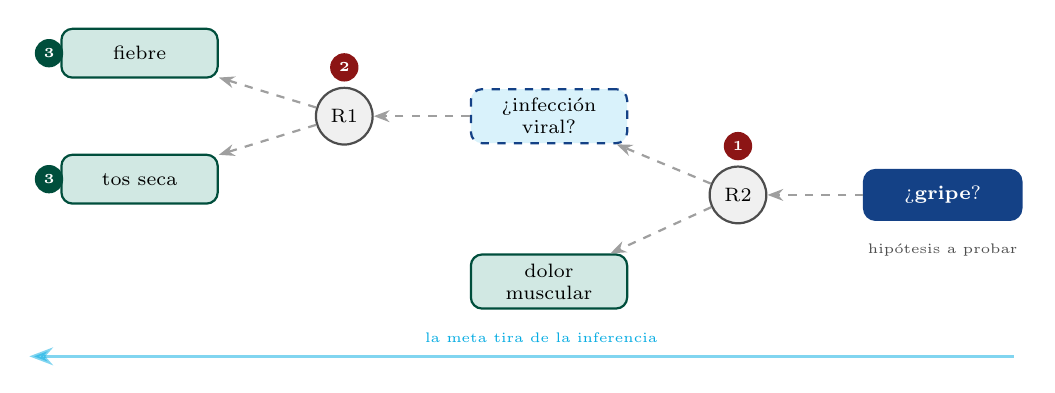
\begin{tikzpicture}[font=\scriptsize,
	hecho/.style={rectangle, draw=AccentGreen!60!black, thick, rounded corners,
		fill=AccentGreen!18, align=center, text width=1.75cm, minimum height=0.62cm},
	sub/.style={rectangle, draw=UCMNavy, thick, rounded corners, dashed,
		fill=UCMBlue!15, align=center, text width=1.75cm, minimum height=0.62cm},
	meta/.style={rectangle, draw=UCMNavy, very thick, rounded corners,
		fill=UCMNavy, text=white, align=center, text width=1.75cm, minimum height=0.62cm},
	regla/.style={circle, draw=StanfordGray, thick, fill=LightGray, minimum size=0.72cm},
	paso/.style={circle, fill=StanfordRed, text=white, inner sep=1pt,
		minimum size=0.36cm, font=\tiny\bfseries},
	fl/.style={-{Stealth[length=2mm]}, thick, gray!75, dashed}]

	\node[meta]  (g)  at (10.2,-0.25) {¿\textbf{gripe}?};
	\node[regla] (r2) at (7.6,-0.25) {R2};
	\node[sub]   (v)  at (5.2,0.75) {¿infecci\'on viral?};
	\node[hecho] (f3) at (5.2,-1.35) {dolor muscular};
	\node[regla] (r1) at (2.6,0.75) {R1};
	\node[hecho] (f1) at (0,1.55) {fiebre};
	\node[hecho] (f2) at (0,-0.05) {tos seca};

	\draw[fl] (g)  -- (r2);
	\draw[fl] (r2) -- (v);    \draw[fl] (r2) -- (f3);
	\draw[fl] (v)  -- (r1);
	\draw[fl] (r1) -- (f1);   \draw[fl] (r1) -- (f2);

	\node[paso] at ($(r2)+(0,0.62)$) {1};
	\node[paso] at ($(r1)+(0,0.62)$) {2};
	\node[paso, fill=AccentGreen!60!black] at ($(f1)+(-1.15,0)$) {3};
	\node[paso, fill=AccentGreen!60!black] at ($(f2)+(-1.15,0)$) {3};

	\node[anchor=north, font=\tiny, text=StanfordGray] at (10.2,-0.75) {hip\'otesis a probar};
	\draw[{Stealth[length=3mm]}-, very thick, UCMBlue, opacity=0.5] (-1.4,-2.3) -- (11.1,-2.3);
	\node[UCMBlue, font=\tiny, anchor=south] at (5.1,-2.25) {la meta tira de la inferencia};
\end{tikzpicture}
\end{center}
\vspace{0.2em}
\begin{itemize}
	\item Parte de una \textbf{hip\'otesis} y busca reglas que la concluyan; sus antecedentes se vuelven nuevas submetas, hasta topar con hechos conocidos o preguntarle al usuario.
	\item Conviene cuando hay \textbf{pocas hip\'otesis y muchos datos posibles}: diagn\'ostico m\'edico o de fallas. Es lo que hac\'ia MYCIN.
\end{itemize}
\end{frame}

\begin{frame}
\frametitle{¿Cuál de las dos estrategias?}
\begin{center}
\begin{tabular}{lll}
\toprule
 & \textbf{Hacia adelante} & \textbf{Hacia atr\'as} \\
\midrule
Dirigido por      & los datos            & la meta \\
Punto de partida  & hechos observados    & hip\'otesis \\
Pregunta al usuario & rara vez           & solo lo que necesita \\
Bueno cuando      & pocos datos, muchas conclusiones & muchos datos, pocas hip\'otesis \\
Riesgo t\'ipico   & derivar hechos in\'utiles & explorar ramas que fracasan \\
Ejemplo           & configuraci\'on (XCON) & diagn\'ostico (MYCIN) \\
\bottomrule
\end{tabular}
\end{center}
\vspace{0.8em}
\begin{itemize}
	\item Ambas usan \textbf{la misma base de reglas}: cambia solo la estrategia de control del motor.
	\item Es exactamente la separaci\'on conocimiento/control de la que hablamos al principio.
\end{itemize}
\end{frame}

\begin{frame}
\frametitle{Razonar con incertidumbre: factores de certeza}
El conocimiento cl\'inico rara vez es categ\'orico. MYCIN asociaba a cada regla un \textbf{factor de certeza} $\mathrm{CF} \in [-1, 1]$.
\vspace{0.3em}
\begin{columns}[T]
\begin{column}{6.4cm}
\regla{R1 con certeza}{\textbf{SI} fiebre \textbf{Y} tos seca\\ \textbf{ENTONCES} infecci\'on viral \quad ($\mathrm{CF}=0{,}7$)}
\vspace{0.2em}
\formula{\footnotesize
\[
\mathrm{CF}(\text{concl.}) = \min_i \mathrm{CF}(\text{premisa}_i)\times \mathrm{CF}(\text{regla})
\]}
\formula{\footnotesize
\[
\mathrm{CF}_{1,2} = \mathrm{CF}_1 + \mathrm{CF}_2\,(1-\mathrm{CF}_1) \quad (\mathrm{CF}_i>0)
\]}
\end{column}
\begin{column}{5.6cm}
\footnotesize
\textbf{Traza del caso:}
\begin{enumerate}
	\item $\mathrm{CF}(\text{fiebre})=1{,}0$, $\mathrm{CF}(\text{tos seca})=0{,}8$
	\item premisa: $\min(1{,}0;\,0{,}8)=0{,}8$
	\item R1: $0{,}8\times 0{,}7 = \mathbf{0{,}56}$
	\item otra regla aporta $0{,}4$ a la misma conclusi\'on
	\item combinadas: $0{,}56 + 0{,}4(1-0{,}56)=\mathbf{0{,}736}$
\end{enumerate}
\end{column}
\end{columns}
\vspace{-0.2em}
\idea{Los factores de certeza fueron una soluci\'on \emph{de ingenier\'ia}, no probabil\'istica: no satisfacen los axiomas de Kolmogorov. Las \textbf{redes bayesianas}, que vemos a continuaci\'on, son la respuesta formal al mismo problema.}
\end{frame}

%=====================================================================
\section{Modelos gráficos probabilísticos}
%=====================================================================

\begin{frame}
\frametitle{Del factor de certeza a la probabilidad}
\begin{columns}[T]
\begin{column}{6.1cm}
\begin{alertblock}{Lo que falla en los CF}
\footnotesize
\begin{itemize}
	\item No hay una semántica: $\mathrm{CF}=0{,}7$ no es un número comprobable contra el mundo.
	\item La combinación supone evidencia \textbf{independiente}: si dos reglas leen el mismo síntoma, se cuenta dos veces.
	\item El razonamiento no se puede invertir: de $\mathrm{CF}$(síntoma $\to$ enfermedad) no se recupera el sentido contrario.
\end{itemize}
\end{alertblock}
\end{column}
\begin{column}{6.1cm}
\begin{block}{La alternativa formal}
\footnotesize
Modelar el dominio con una \textbf{distribución conjunta}. Con $E$ la enfermedad y $S$ los síntomas, toda pregunta es marginalizar y condicionar:
\vspace{-0.4em}
\[
P(E \mid S) \;=\; \frac{P(E, S)}{P(S)}
\]
\vspace{-1.2em}
\end{block}
\vspace{-0.2em}
\formula{\footnotesize\centering Regla de la cadena:\\[3pt]
$\displaystyle P(X_1,\dots,X_n)=\prod_{i=1}^{n} P(X_i \mid X_{<i})$\\[3pt]
{\scriptsize con $X_{<i} = \{X_1,\dots,X_{i-1}\}$}}
\end{column}
\end{columns}
\vspace{0.2em}
\idea{Correcto pero inviable: la conjunta sobre $n$ variables binarias necesita $2^{n}-1$ números; con $n=30$ son mil millones que nadie puede estimar ni almacenar. Hace falta \textbf{estructura}.}
\end{frame}

\begin{frame}
\frametitle{Modelos gráficos probabilísticos}
\begin{block}{Idea}
\footnotesize
Usar un \textbf{grafo} para declarar qué variables interactúan \emph{directamente}. Los nodos son variables aleatorias; la ausencia de una arista es una afirmación de \textbf{independencia condicional}. El grafo hace dos cosas a la vez: \textbf{factoriza} la conjunta y \textbf{codifica} independencias.
\end{block}
\vspace{0.2em}
\begin{columns}[T]
\begin{column}{6.1cm}
\begin{center}
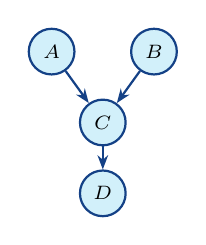
\begin{tikzpicture}[font=\scriptsize,
	v/.style={circle, draw=UCMNavy, thick, fill=UCMBlue!18, minimum size=0.58cm, inner sep=0pt},
	fl/.style={-{Stealth[length=1.8mm]}, thick, UCMNavy}]
	\node[v] (a) at (0,1.0) {$A$};
	\node[v] (b) at (1.3,1.0) {$B$};
	\node[v] (c) at (0.65,0.1) {$C$};
	\node[v] (d) at (0.65,-0.8) {$D$};
	\draw[fl] (a)--(c); \draw[fl] (b)--(c); \draw[fl] (c)--(d);
\end{tikzpicture}
\end{center}
\footnotesize
\textbf{Dirigidos --- redes bayesianas}\\
Aristas con dirección y sin ciclos: dependencia \emph{asimétrica}, a menudo causal. Factorizan en probabilidades condicionales, ya normalizadas.
\end{column}
\begin{column}{6.1cm}
\begin{center}
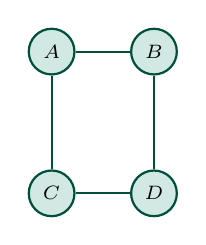
\begin{tikzpicture}[font=\scriptsize,
	v/.style={circle, draw=AccentGreen!60!black, thick, fill=AccentGreen!18, minimum size=0.58cm, inner sep=0pt},
	ln/.style={thick, AccentGreen!60!black}]
	\node[v] (a) at (0,1.0) {$A$};
	\node[v] (b) at (1.3,1.0) {$B$};
	\node[v] (c) at (0,-0.8) {$C$};
	\node[v] (d) at (1.3,-0.8) {$D$};
	\draw[ln] (a)--(b); \draw[ln] (a)--(c); \draw[ln] (b)--(d); \draw[ln] (c)--(d);
\end{tikzpicture}
\end{center}
\footnotesize
\textbf{No dirigidos --- campos de Markov}\\
Aristas simétricas. Factorizan en \emph{potenciales} sobre cliques, con una constante global $Z$ que suele ser intratable. Útiles cuando no hay dirección natural.
\end{column}
\end{columns}
\vspace{0.1em}
\footnotesize En esta clase nos quedamos con los \textbf{dirigidos}: son los que reemplazan al motor de reglas con incertidumbre.
\end{frame}

\begin{frame}
\frametitle{Red bayesiana: definición}
\begin{block}{Definición}
\footnotesize
Una \textbf{red bayesiana} sobre $X_1,\dots,X_n$ es un par $(\mathcal{G}, \Theta)$: un \textbf{grafo dirigido acíclico} (DAG) con un nodo por variable ---escribimos $\Pa(X_i)$ para los padres de $X_i$--- y una \textbf{distribución condicional} $P(X_i \mid \Pa(X_i))$ por nodo (si es discreta, una tabla: una CPT).
\end{block}
\vspace{-0.1em}
\formula{\centering \textbf{Semántica: regla de la cadena para redes bayesianas}\\[3pt]
$\displaystyle P(X_1,\dots,X_n) \;=\; \prod_{i=1}^{n} P\bigl(X_i \,\big|\, \Pa(X_i)\bigr)$}
\vspace{-0.1em}
\begin{columns}[T]
\begin{column}{6.1cm}
\footnotesize
\textbf{Cómo leerla.} Es la regla de la cadena en la que cada conjunto condicionante $\{X_1,\dots,X_{i-1}\}$ se ha \emph{podado} hasta dejar solo los padres. La red es exactamente esa lista de podas.
\end{column}
\begin{column}{6.1cm}
\footnotesize
\textbf{Afirmación equivalente (Markov local).}
\vspace{-0.4em}
\[
X_i \;\indep\; \mathrm{NoDesc}(X_i) \;\big|\; \Pa(X_i)
\]
\vspace{-1.1em}

Dados sus padres, un nodo es independiente de todo lo que no sea descendiente suyo.
\end{column}
\end{columns}
\vspace{0.1em}
\idea{Factorizar e independizar son \textbf{la misma afirmación}: $P$ factoriza sobre $\mathcal{G}$ si y solo si $P$ satisface la propiedad de Markov local de $\mathcal{G}$.}
\end{frame}

\begin{frame}
\frametitle{Un ejemplo clínico}
\begin{columns}[T]
\begin{column}{5.5cm}
\vspace{0.3em}
\begin{center}
\scalebox{0.92}{%
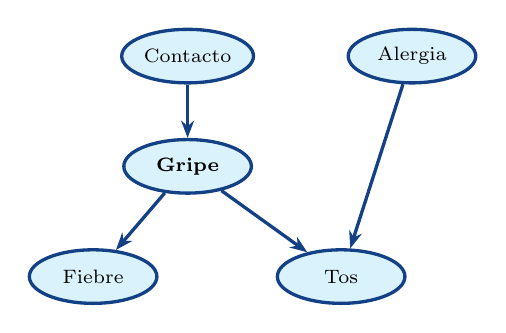
\begin{tikzpicture}[font=\scriptsize,
	v/.style={ellipse, draw=UCMNavy, very thick, fill=UCMBlue!15,
		minimum width=1.62cm, minimum height=0.68cm, inner sep=1pt},
	fl/.style={-{Stealth[length=2.2mm]}, very thick, UCMNavy}]
	\node[v] (C) at (0,2.3)     {Contacto};
	\node[v] (A) at (2.85,2.3)  {Alergia};
	\node[v] (G) at (0,0.9)     {\textbf{Gripe}};
	\node[v] (F) at (-1.2,-0.5) {Fiebre};
	\node[v] (T) at (1.95,-0.5) {Tos};
	\draw[fl] (C) -- (G);
	\draw[fl] (G) -- (F);
	\draw[fl] (G) -- (T);
	\draw[fl] (A) -- (T);
\end{tikzpicture}}
\end{center}
\vspace{0.2em}
\formula{\scriptsize\centering
$P(C,A,G,F,T)=$\\[2pt]
$P(C)\,P(A)\,P(G|C)\,P(F|G)\,P(T|G,A)$}
\end{column}
\begin{column}{6.7cm}
\scriptsize
\vspace{0.2em}
\begin{columns}[T]
\begin{column}{2.6cm}
\begin{tabular}{@{}lc@{}}
\toprule
\multicolumn{2}{@{}l}{$P(C)$}\\
\midrule
sí & $0{,}10$\\
\bottomrule
\end{tabular}

\vspace{0.5em}
\begin{tabular}{@{}lc@{}}
\toprule
\multicolumn{2}{@{}l}{$P(A)$}\\
\midrule
sí & $0{,}20$\\
\bottomrule
\end{tabular}

\vspace{0.5em}
\begin{tabular}{@{}lc@{}}
\toprule
$C$ & $P(G{=}\text{sí}|C)$\\
\midrule
sí & $0{,}40$\\
no & $0{,}02$\\
\bottomrule
\end{tabular}
\end{column}
\begin{column}{3.5cm}
\begin{tabular}{@{}lc@{}}
\toprule
$G$ & $P(F{=}\text{sí}|G)$\\
\midrule
sí & $0{,}90$\\
no & $0{,}05$\\
\bottomrule
\end{tabular}

\vspace{0.5em}
\begin{tabular}{@{}llc@{}}
\toprule
$G$ & $A$ & $P(T{=}\text{sí}|G,A)$\\
\midrule
sí & sí & $0{,}95$\\
sí & no & $0{,}85$\\
no & sí & $0{,}70$\\
no & no & $0{,}05$\\
\bottomrule
\end{tabular}
\end{column}
\end{columns}
\end{column}
\end{columns}
\vspace{0.3em}
\footnotesize Las cinco variables son binarias. El grafo dice, por ejemplo, que \emph{el contacto solo importa a través de la gripe} y que \emph{la alergia no afecta a la fiebre}.
\end{frame}

\begin{frame}
\frametitle{La semántica en acción: cuánto se ahorra}
\begin{columns}[T]
\begin{column}{6.2cm}
\textbf{Evaluar una entrada de la conjunta} es multiplicar cinco números locales:
\vspace{-0.2em}
{\footnotesize
\begin{align*}
&P(c,\lnot a, g, f, t) \\[2pt]
&= \underbrace{0{,}10}_{P(c)}\cdot \underbrace{0{,}80}_{P(\lnot a)}\cdot \underbrace{0{,}40}_{P(g|c)}\cdot \underbrace{0{,}90}_{P(f|g)}\cdot \underbrace{0{,}85}_{P(t|g\lnot a)}\\[2pt]
&= 0{,}0245
\end{align*}}
\vspace{-0.6em}
\begin{center}
\scriptsize
\begin{tabular}{@{}lcc@{}}
\toprule
 & \textbf{conjunta plena} & \textbf{red bayesiana}\\
\midrule
$n=5$   & $31$      & $\mathbf{10}$\\
$n=10$  & $1\,023$  & $\sim\!30$\\
$n=30$  & $10^{9}$  & $\sim\!100$\\
\bottomrule
\end{tabular}
\end{center}
\end{column}
\begin{column}{6.0cm}
\begin{block}{De dónde sale el ahorro}
\footnotesize
Un nodo con $k$ padres binarios cuesta $2^{k}$ parámetros, no $2^{n-1}$. El costo total es
\[
\sum_{i=1}^{n} 2^{|\Pa(X_i)|}
\quad\text{en vez de}\quad 2^{n}-1 .
\]
Si el número de padres está acotado por $k$, la red es \textbf{lineal} en $n$: $\mathcal{O}(n\,2^{k})$.
\end{block}
\vspace{-0.2em}
\begin{alertblock}{El precio}
\footnotesize
El ahorro es exactamente el conjunto de independencias que hemos \emph{afirmado}. Si una de ellas es falsa en el dominio, el modelo está mal, no solo comprimido.
\end{alertblock}
\end{column}
\end{columns}
\end{frame}

\begin{frame}
\frametitle{Estructura e independencia: las tres conexiones}
Toda ruta entre dos nodos pasa por uno de estos tres patrones. Verde $=$ variable \textbf{observada}.
\vspace{0.4em}
\begin{center}
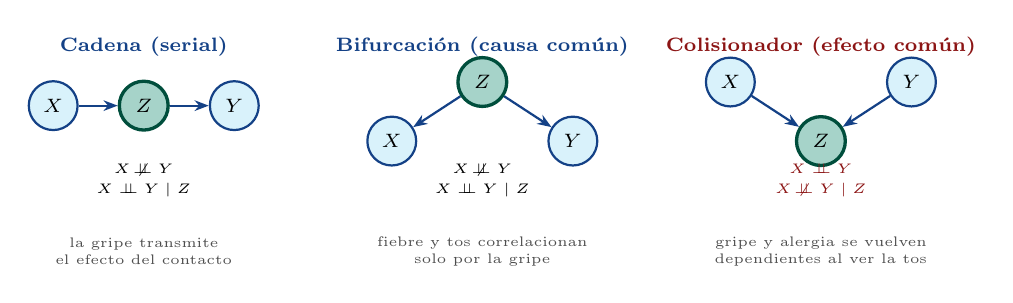
\begin{tikzpicture}[font=\scriptsize,
	v/.style={circle, draw=UCMNavy, thick, fill=UCMBlue!15, minimum size=0.62cm, inner sep=0pt},
	obs/.style={circle, draw=AccentGreen!60!black, very thick, fill=AccentGreen!35, minimum size=0.62cm, inner sep=0pt},
	fl/.style={-{Stealth[length=1.8mm]}, thick, UCMNavy}]

	% --- cadena ---
	\begin{scope}[xshift=0cm]
		\node[font=\scriptsize\bfseries, text=UCMNavy] at (1.15,1.35) {Cadena (serial)};
		\node[v] (x1) at (0,0.6) {$X$};
		\node[obs] (z1) at (1.15,0.6) {$Z$};
		\node[v] (y1) at (2.3,0.6) {$Y$};
		\draw[fl] (x1)--(z1); \draw[fl] (z1)--(y1);
		\node[font=\tiny, align=center] at (1.15,-0.35) {$X \nindep Y$\\[1pt] $X \indep Y \mid Z$};
		\node[font=\tiny, text=StanfordGray, align=center] at (1.15,-1.25) {la gripe transmite\\ el efecto del contacto};
	\end{scope}
	% --- bifurcación ---
	\begin{scope}[xshift=4.3cm]
		\node[font=\scriptsize\bfseries, text=UCMNavy] at (1.15,1.35) {Bifurcación (causa común)};
		\node[v] (x2) at (0,0.15) {$X$};
		\node[obs] (z2) at (1.15,0.9) {$Z$};
		\node[v] (y2) at (2.3,0.15) {$Y$};
		\draw[fl] (z2)--(x2); \draw[fl] (z2)--(y2);
		\node[font=\tiny, align=center] at (1.15,-0.35) {$X \nindep Y$\\[1pt] $X \indep Y \mid Z$};
		\node[font=\tiny, text=StanfordGray, align=center] at (1.15,-1.25) {fiebre y tos correlacionan\\ solo por la gripe};
	\end{scope}
	% --- colisionador ---
	\begin{scope}[xshift=8.6cm]
		\node[font=\scriptsize\bfseries, text=StanfordRed] at (1.15,1.35) {Colisionador (efecto común)};
		\node[v] (x3) at (0,0.9) {$X$};
		\node[obs] (z3) at (1.15,0.15) {$Z$};
		\node[v] (y3) at (2.3,0.9) {$Y$};
		\draw[fl] (x3)--(z3); \draw[fl] (y3)--(z3);
		\node[font=\tiny, align=center, text=StanfordRed] at (1.15,-0.35) {$X \indep Y$\\[1pt] $X \nindep Y \mid Z$};
		\node[font=\tiny, text=StanfordGray, align=center] at (1.15,-1.25) {gripe y alergia se vuelven\\ dependientes al ver la tos};
	\end{scope}
\end{tikzpicture}
\end{center}
\vspace{0.5em}
\idea{Condicionar \textbf{bloquea} una cadena y una bifurcación, pero \textbf{abre} un colisionador. Es el único caso en que observar una variable crea dependencia donde no la había, y es la razón de que la lectura ingenua ``más evidencia, más independencia'' sea falsa.}
\end{frame}

\begin{frame}
\frametitle{El colisionador con números: \emph{explaining away}}
\begin{columns}[T]
\begin{column}{6.4cm}
Sobre la red del ejemplo, seguimos la creencia en \textbf{gripe}:
\vspace{0.3em}
\begin{center}
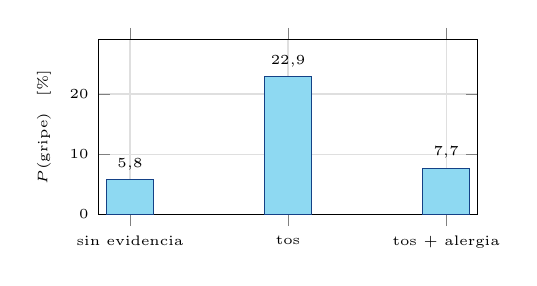
\begin{tikzpicture}[font=\scriptsize]
\begin{axis}[width=6.4cm, height=3.8cm,
	ybar, bar width=17pt,
	symbolic x coords={sin evidencia, tos, {tos + alergia}},
	xtick=data, x tick label style={font=\tiny, align=center},
	ylabel={$P(\text{gripe})$ \, [\%]}, ylabel style={font=\tiny},
	tick label style={font=\tiny}, ymin=0, ymax=29,
	nodes near coords,
	every node near coord/.append style={font=\tiny,
		/pgf/number format/fixed, /pgf/number format/precision=1,
		/pgf/number format/use comma},
	grid=major, grid style={gray!25}]
	\addplot[fill=UCMBlue!45, draw=UCMNavy] coordinates
		{(sin evidencia,5.8) (tos,22.9) ({tos + alergia},7.7)};
\end{axis}
\end{tikzpicture}
\end{center}
\end{column}
\begin{column}{5.8cm}
\footnotesize
\begin{itemize}
	\item A priori, $P(G)=0{,}058$.
	\item Observar \textbf{tos} sube la creencia a $0{,}229$: la tos es evidencia de gripe.
	\item Observar además que el paciente es \textbf{alérgico} la baja a $0{,}077$: la alergia \emph{ya explica} la tos, así que la gripe deja de hacer falta.
\end{itemize}
\vspace{0.3em}
\begin{block}{Por qué importa}
\footnotesize
Un motor de reglas con factores de certeza no puede hacer esto: sus reglas solo \emph{suman} evidencia a favor. Aquí una evidencia \textbf{resta} creencia a una hipótesis rival sin que nadie escribiera una regla para ello: sale de la estructura.
\end{block}
\end{column}
\end{columns}
\end{frame}

\begin{frame}
\frametitle{d-separación: el criterio general}
\begin{block}{Ruta bloqueada}
Una ruta (no dirigida) entre $X$ e $Y$ está \textbf{bloqueada} por un conjunto de evidencia $\mathbf{Z}$ si contiene algún nodo $W$ tal que:
\end{block}
\vspace{-0.2em}
\begin{center}
\footnotesize
\begin{tabular}{@{}ll@{}}
\toprule
\textbf{Patrón en la ruta} & \textbf{Bloquea cuando} \\
\midrule
cadena \;$\rightarrow W \rightarrow$\; o bifurcación \;$\leftarrow W \rightarrow$\; & $W \in \mathbf{Z}$ \\
colisionador \;$\rightarrow W \leftarrow$\; & $W \notin \mathbf{Z}$ \; \textbf{y} ningún descendiente de $W$ está en $\mathbf{Z}$ \\
\bottomrule
\end{tabular}
\end{center}
\vspace{0.4em}
\formula{\centering
$X \;\text{d-separado de}\; Y \;\text{dado}\; \mathbf{Z}$ \;$\Longrightarrow$\; $X \indep Y \mid \mathbf{Z}$ \; en toda $P$ que factorice sobre $\mathcal{G}$}
\vspace{0.3em}
\begin{columns}[T]
\begin{column}{6.1cm}
\footnotesize
\textbf{Todas} las rutas deben estar bloqueadas: basta una abierta para que el grafo no garantice independencia.
\end{column}
\begin{column}{6.1cm}
\footnotesize
\textbf{Cuidado con los descendientes.} Si la tos provoca \emph{consulta médica} y observamos la consulta, el colisionador se abre igual.
\end{column}
\end{columns}
\vspace{0.1em}
\idea{La d-separación convierte una pregunta probabilística en un problema de \textbf{caminos en un grafo}: se responde mirando el dibujo, sin tocar un solo número.}
\end{frame}

\begin{frame}
\frametitle{Manto de Markov}
\begin{columns}[c]
\begin{column}{5.6cm}
\begin{center}
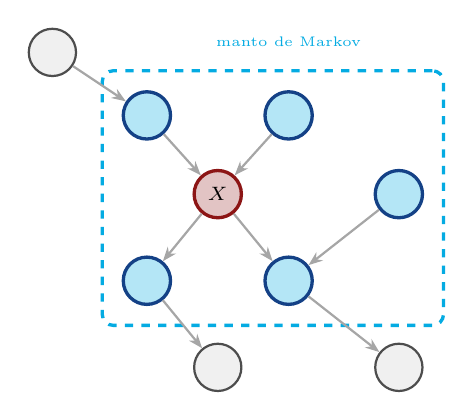
\begin{tikzpicture}[font=\scriptsize,
	v/.style={circle, draw=StanfordGray, thick, fill=LightGray, minimum size=0.6cm, inner sep=0pt},
	mb/.style={circle, draw=UCMNavy, very thick, fill=UCMBlue!30, minimum size=0.6cm, inner sep=0pt},
	me/.style={circle, draw=StanfordRed, very thick, fill=StanfordRed!25, minimum size=0.6cm, inner sep=0pt},
	fl/.style={-{Stealth[length=1.8mm]}, thick, gray!70}]

	\node[mb] (p1) at (-0.9,1.3) {};
	\node[mb] (p2) at (0.9,1.3) {};
	\node[me] (x)  at (0,0.3) {$X$};
	\node[mb] (h1) at (-0.9,-0.8) {};
	\node[mb] (h2) at (0.9,-0.8) {};
	\node[mb] (cp) at (2.3,0.3) {};
	\node[v]  (g1) at (-2.1,2.1) {};
	\node[v]  (g2) at (0,-1.9) {};
	\node[v]  (g3) at (2.3,-1.9) {};

	\draw[fl] (p1)--(x); \draw[fl] (p2)--(x);
	\draw[fl] (x)--(h1); \draw[fl] (x)--(h2);
	\draw[fl] (cp)--(h2);
	\draw[fl] (g1)--(p1); \draw[fl] (h1)--(g2); \draw[fl] (h2)--(g3);

	\begin{scope}[on background layer]
		\node[draw=UCMBlue, dashed, very thick, rounded corners, inner sep=7pt,
			fit=(p1)(p2)(x)(h1)(h2)(cp)] {};
	\end{scope}
	\node[font=\tiny, text=UCMBlue, anchor=south] at (0.9,2.05) {manto de Markov};
\end{tikzpicture}
\end{center}
\end{column}
\begin{column}{6.4cm}
\begin{block}{Definición}
El \textbf{manto de Markov} de $X$ es el conjunto formado por:
\begin{itemize}
	\item sus \textbf{padres},
	\item sus \textbf{hijos},
	\item los \textbf{otros padres de sus hijos}.
\end{itemize}
\end{block}
\vspace{-0.1em}
\formula{\centering $X \;\indep\; \text{resto de la red} \;\big|\; \mathrm{MB}(X)$}
\vspace{-0.1em}
\footnotesize
Los otros padres entran porque cada hijo es un \textbf{colisionador}: observarlo abre la ruta hacia ellos.
\end{column}
\end{columns}
\vspace{0.3em}
\idea{El manto es la ``interfaz'' de una variable con el resto del modelo: para actualizar $X$ basta mirar su vecindad. Es lo que hace local el cómputo en muestreo de Gibbs y en propagación de creencias.}
\end{frame}

\begin{frame}
\frametitle{Qué afirma el grafo (y qué no)}
\begin{columns}[T]
\begin{column}{6.1cm}
\begin{block}{El grafo es un \emph{I-map}}
\footnotesize
Toda independencia que el grafo declara (por d-separación) se cumple en $P$. Lo recíproco \textbf{no} vale: $P$ puede tener independencias adicionales que el grafo no muestra.
\end{block}
\vspace{-0.2em}
\begin{alertblock}{Consecuencias prácticas}
\footnotesize
\begin{itemize}
	\item Una \textbf{arista de más} nunca hace incorrecto el modelo: solo lo hace más caro y más difícil de estimar.
	\item Una \textbf{arista de menos} sí lo hace incorrecto: afirma una independencia falsa.
	\item El grafo completo es un I-map de cualquier $P$, y es inútil.
	\item No siempre existe un \emph{P-map}: hay distribuciones cuyo conjunto exacto de independencias ningún DAG reproduce.
\end{itemize}
\end{alertblock}
\end{column}
\begin{column}{6.1cm}
\textbf{El orden de las variables importa.} La misma distribución, construida con dos órdenes distintos:
\vspace{0.3em}
\begin{center}
\scalebox{0.74}{%
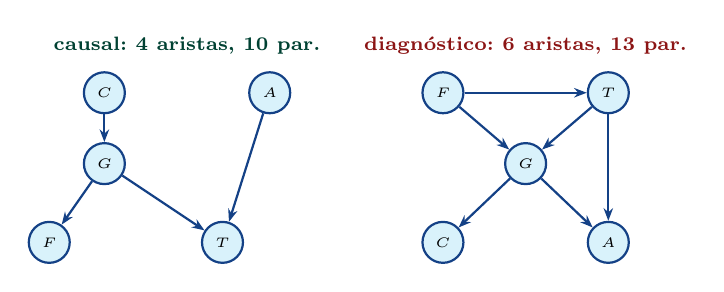
\begin{tikzpicture}[font=\tiny,
	v/.style={circle, draw=UCMNavy, thick, fill=UCMBlue!15, minimum size=0.52cm, inner sep=0pt},
	fl/.style={-{Stealth[length=1.6mm]}, thick, UCMNavy}]
	% causal
	\begin{scope}
		\node[font=\scriptsize\bfseries, text=AccentGreen!50!black] at (1.05,1.9) {causal: 4 aristas, 10 par.};
		\node[v] (C) at (0,1.3) {$C$};   \node[v] (A) at (2.1,1.3) {$A$};
		\node[v] (G) at (0,0.4) {$G$};
		\node[v] (F) at (-0.7,-0.6) {$F$}; \node[v] (T) at (1.5,-0.6) {$T$};
		\draw[fl] (C)--(G); \draw[fl] (G)--(F); \draw[fl] (G)--(T); \draw[fl] (A)--(T);
	\end{scope}
	% diagnóstico
	\begin{scope}[xshift=4.3cm]
		\node[font=\scriptsize\bfseries, text=StanfordRed] at (1.05,1.9) {diagnóstico: 6 aristas, 13 par.};
		\node[v] (F2) at (0,1.3) {$F$};  \node[v] (T2) at (2.1,1.3) {$T$};
		\node[v] (G2) at (1.05,0.4) {$G$};
		\node[v] (A2) at (2.1,-0.6) {$A$}; \node[v] (C2) at (0,-0.6) {$C$};
		\draw[fl] (F2)--(T2); \draw[fl] (F2)--(G2); \draw[fl] (T2)--(G2);
		\draw[fl] (T2)--(A2); \draw[fl] (G2)--(A2); \draw[fl] (G2)--(C2);
	\end{scope}
\end{tikzpicture}}
\end{center}
\vspace{0.2em}
\footnotesize Ambas representan \emph{la misma} conjunta. Ordenar de causas a efectos produce el grafo más disperso y las tablas más fáciles de rellenar.
\end{column}
\end{columns}
\end{frame}

\begin{frame}
\frametitle{Preguntarle a la red: inferencia}
\begin{columns}[T]
\begin{column}{6.1cm}
\begin{block}{Tipos de consulta}
\footnotesize
\begin{itemize}
	\item \textbf{Marginal a posteriori}: $P(G \mid F{=}\text{sí}, T{=}\text{sí})$.
	\item \textbf{MAP}: la asignación conjunta más probable de las variables no observadas.
	\item \textbf{Diagnóstico} (efecto $\to$ causa) y \textbf{predicción} (causa $\to$ efecto) usan \emph{el mismo} modelo: la red no tiene una dirección privilegiada de uso, a diferencia del motor de reglas.
\end{itemize}
\end{block}
\end{column}
\begin{column}{6.1cm}
\begin{block}{Cómo se calcula}
\footnotesize
\begin{itemize}
	\item \textbf{Exacta}: eliminación de variables, árbol de uniones. Costo exponencial en el \emph{ancho de árbol} del grafo, no en $n$.
	\item \textbf{Aproximada}: muestreo (rechazo, ponderación por verosimilitud, Gibbs) o métodos variacionales.
	\item El problema general es \textbf{NP-difícil}, también en su versión aproximada. En la práctica se explota que las redes reales son dispersas.
\end{itemize}
\end{block}
\end{column}
\end{columns}
\vspace{0.3em}
\footnotesize Herramientas: \texttt{pgmpy} (Python), \texttt{bnlearn} (R), SamIam y GeNIe para modelar y consultar de forma interactiva.
\vspace{0.2em}
\idea{Una red bayesiana es una \textbf{base de conocimiento declarativa} como la de un sistema experto, pero con una semántica probabilística: el motor de inferencia deja de encadenar reglas y pasa a marginalizar.}
\end{frame}

\begin{frame}
\frametitle{Cómo modelar una situación real: receta}
\footnotesize
\begin{columns}[T]
\begin{column}{6.1cm}
\begin{enumerate}
	\item \textbf{Escribe primero la consulta.} ¿Qué se va a preguntar y qué se va a observar? Eso decide qué variables existen; todo lo demás sobra.
	\item \textbf{Define las variables.} Estados \textbf{exhaustivos y mutuamente excluyentes}. Prefiere pocos estados: cada uno multiplica el tamaño de las CPT de los hijos.
	\item \textbf{Ordena de causas a efectos.} Enfermedad antes que síntoma, falla antes que alarma. Ese orden da el grafo más disperso.
	\item \textbf{Dibuja las aristas.} Para cada par, pregunta: \emph{conocidos los padres ya elegidos, ¿saber $X$ cambia mi creencia sobre $Y$?} Si no, no hay arista.
\end{enumerate}
\end{column}
\begin{column}{6.1cm}
\begin{enumerate}
	\setcounter{enumi}{4}
	\item \textbf{Verifica las independencias implicadas.} Recorre las aristas ausentes y comprueba con d-separación que lo que afirmas es defendible en el dominio.
	\item \textbf{Rellena las CPT.} Datos donde los haya; elicitación experta donde no. Con muchos padres, usa modelos canónicos (\emph{noisy-OR}, \emph{noisy-MAX}) que necesitan $k$ números en vez de $2^{k}$.
	\item \textbf{Valida.} Casos extremos (todo presente / todo ausente), análisis de sensibilidad, y comprueba que aparece el \emph{explaining away} donde el experto lo espera.
\end{enumerate}
\end{column}
\end{columns}
\vspace{0.4em}
\idea{Modelar es iterar entre los pasos 4 y 7. La primera red nunca es la buena; lo valioso es que cada corrección es \textbf{local}: se toca un nodo y sus tablas, no todo el sistema.}
\end{frame}

\begin{frame}
\frametitle{Errores frecuentes al modelar}
\begin{columns}[T]
\begin{column}{6.1cm}
\begin{alertblock}{Aristas en dirección diagnóstica}
\footnotesize
Dibujar \emph{síntoma $\to$ enfermedad} porque así razona el médico: la enfermedad acumula decenas de padres y las CPT explotan. Dibuja la causalidad; la inferencia ya invierte sola.
\end{alertblock}
\begin{alertblock}{Confundir arista con correlación}
\footnotesize
Dos variables correlacionadas pueden no necesitar arista si una causa común ya explica la asociación.
\end{alertblock}
\begin{alertblock}{Discretizar demasiado fino}
\footnotesize
Diez niveles de temperatura con tres padres son $10\cdot 2^3$ celdas que rellenar. Usa los cortes que el experto distingue.
\end{alertblock}
\end{column}
\begin{column}{6.1cm}
\begin{alertblock}{Olvidar las variables latentes}
\footnotesize
Si dos síntomas correlacionan sin causa modelada, la red los hará depender por caminos absurdos. Suele faltar un nodo no observable que capture la causa común.
\end{alertblock}
\begin{alertblock}{Sesgo de selección}
\footnotesize
Con datos de pacientes ya hospitalizados se condiciona sobre un \textbf{colisionador} (\emph{ingresó al hospital}): aparecen dependencias espurias entre enfermedades independientes en la población.
\end{alertblock}
\begin{block}{Regla de bolsillo}
\footnotesize
Ante la duda, \textbf{añade} la arista: sobran parámetros, pero no miente.
\end{block}
\end{column}
\end{columns}
\end{frame}

%=====================================================================
\section{Historia, límites y legado}
%=====================================================================

\begin{frame}
\frametitle{Auge y caída, en una lámina}
\begin{center}
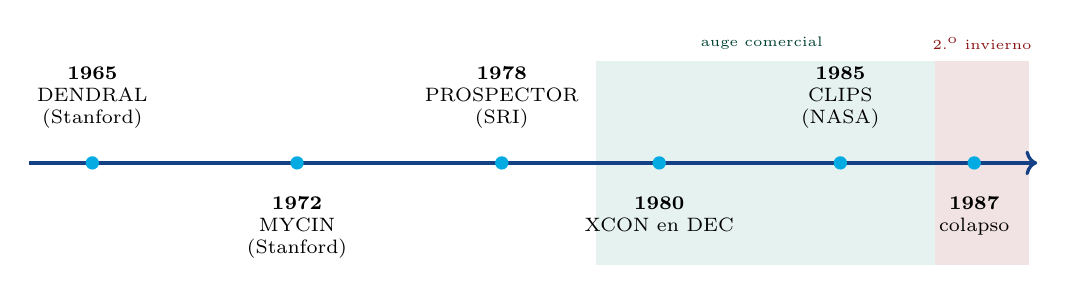
\begin{tikzpicture}[font=\scriptsize, hito/.style={circle, fill=UCMBlue, inner sep=1.7pt}]
	\begin{scope}[on background layer]
		\fill[AccentGreen, opacity=0.10] (6.8,-1.3) rectangle (11.1,1.3);
		\fill[StanfordRed, opacity=0.12] (11.1,-1.3) rectangle (12.3,1.3);
	\end{scope}
	\draw[->, very thick, UCMNavy] (-0.4,0) -- (12.4,0);

	\foreach \x/\a/\t [count=\i] in {
		0.4/1965/{DENDRAL\\(Stanford)},
		3.0/1972/{MYCIN\\(Stanford)},
		5.6/1978/{PROSPECTOR\\(SRI)},
		7.6/1980/{XCON en DEC},
		9.9/1985/{CLIPS\\(NASA)},
		11.6/1987/{colapso}}{
		\node[hito] (h\i) at (\x,0) {};
		\ifodd\i
			\node[above=2.2mm of h\i, align=center, font=\scriptsize] {\textbf{\a}\\\t};
		\else
			\node[below=2.2mm of h\i, align=center, font=\scriptsize] {\textbf{\a}\\\t};
		\fi
	}
	\node[AccentGreen!50!black, font=\tiny, anchor=south] at (8.9,1.32) {auge comercial};
	\node[StanfordRed, font=\tiny, anchor=south] at (11.7,1.32) {2.\textsuperscript{o} invierno};
\end{tikzpicture}
\end{center}
\vspace{0.7em}
\begin{itemize}
	\item \textbf{DENDRAL} (desde 1965) infer\'ia estructuras moleculares a partir de espectrometr\'ia de masas: el primer sistema que codific\'o heur\'isticas de un especialista.
	\item \textbf{MYCIN} (1972--76) diagnosticaba infecciones bacterianas con unas 600 reglas y encadenamiento hacia atr\'as. Igual\'o a especialistas humanos en evaluaciones ciegas y \textbf{nunca se us\'o cl\'inicamente}: problemas de responsabilidad legal y de integraci\'on.
	\item \textbf{XCON} configuraba pedidos de computadores VAX en DEC; creci\'o hasta varios miles de reglas y se le atribuyeron ahorros del orden de decenas de millones de d\'olares al a\~no.
\end{itemize}
\end{frame}

\begin{frame}
\frametitle{Por qué se estancaron}
\begin{columns}[T]
\begin{column}{6.1cm}
\begin{alertblock}{El cuello de botella del conocimiento}
Extraer reglas de un especialista es lento y caro. Buena parte de la pericia es \textbf{t\'acita}: el experto sabe hacerlo, pero no sabe enunciar la regla.
\end{alertblock}
\begin{alertblock}{Mantenimiento}
Con miles de reglas aparecen contradicciones, redundancias y efectos de orden. Cada cambio puede romper conclusiones lejanas.
\end{alertblock}
\end{column}
\begin{column}{6.1cm}
\begin{alertblock}{Fragilidad en los bordes}
Fuera de su dominio no degradan con elegancia: fallan en seco. No tienen sentido com\'un.
\end{alertblock}
\begin{block}{El contraste que vendría}
El aprendizaje autom\'atico ataca exactamente ese cuello de botella: en vez de \emph{entrevistar} al experto, \textbf{induce} las regularidades desde los datos. A cambio, pierde la traza explicativa.
\end{block}
\end{column}
\end{columns}
\vspace{0.4em}
\footnotesize El colapso del mercado de m\'aquinas Lisp hacia 1987 marc\'o el inicio del segundo invierno de la IA que vimos en la clase anterior.
\end{frame}

\begin{frame}
\frametitle{El legado: dónde sobreviven hoy}
\begin{columns}[T]
\begin{column}{6.1cm}
\begin{exampleblock}{Motores de reglas en producción}
CLIPS, Drools y los motores de reglas de negocio siguen operando donde la l\'ogica debe ser \textbf{auditable}: normativa tributaria, seguros, control de procesos.
\end{exampleblock}
\begin{exampleblock}{IA explicable (XAI)}
La capacidad de justificar una conclusi\'on paso a paso, que los sistemas expertos ten\'ian gratis, hoy es un \'area de investigaci\'on activa.
\end{exampleblock}
\end{column}
\begin{column}{6.1cm}
\begin{exampleblock}{Sistemas híbridos y neuro-simbólicos}
Un modelo neuronal propone; un componente simb\'olico verifica contra restricciones duras. Es la arquitectura de los asistentes que llaman herramientas y consultan bases de datos.
\end{exampleblock}
\begin{block}{Lectura para el resto del curso}
Cuando un LLM invoca una herramienta o un verificador, est\'a reponiendo justo lo que el paradigma conexionista no trae: conocimiento \textbf{expl\'icito} y \textbf{comprobable}.
\end{block}
\end{column}
\end{columns}
\end{frame}

%=====================================================================
\section{Cierre}
%=====================================================================

\begin{frame}
\frametitle{Resumen}
\begin{center}
\footnotesize
\begin{tabular}{ll}
\toprule
\textbf{Concepto} & \textbf{Idea clave}\\
\midrule
Sistema experto     & Dominio estrecho + conocimiento declarado expl\'icitamente\\
Arquitectura        & Conocimiento (reglas) separado del control (motor)\\
L\'ogica proposicional & Proposiciones, conectivas y tablas de verdad\\
Modelo              & Una asignaci\'on de verdad; hay $2^n$ de ellas\\
$\rightarrow$ vs.\ $\models$ & Conectiva vs.\ relaci\'on entre conjuntos de modelos\\
Inferencia          & Aplicar reglas en vez de enumerar mundos\\
Encadenamiento      & Adelante: lo empujan los datos. Atr\'as: tira la meta\\
Incertidumbre       & Factores de certeza: ingenier\'ia, no probabilidad\\
Red bayesiana       & DAG $+$ una CPD por nodo: $P(\mathbf{X})=\prod_i P(X_i\mid \Pa(X_i))$\\
Semántica           & Factorizar $\equiv$ afirmar independencias condicionales\\
Tres conexiones     & Cadena y bifurcaci\'on se bloquean al observar; el colisionador se abre\\
d-separaci\'on      & Independencia le\'ida como bloqueo de caminos en el grafo\\
L\'imite            & El cuello de botella de la adquisici\'on de conocimiento\\
\bottomrule
\end{tabular}
\end{center}
\vspace{0.7em}
\begin{itemize}
	\item El conocimiento explícito da \textbf{trazabilidad}; el aprendizaje desde datos da \textbf{escala}. El curso avanza ahora hacia el segundo, sin olvidar lo que se pierde.
	\item Las redes bayesianas est\'an en el medio: conocimiento \textbf{declarativo y auditable}, pero con sem\'antica probabil\'istica y par\'ametros que pueden \textbf{aprenderse de los datos}.
\end{itemize}
\end{frame}

\begin{frame}
\frametitle{Para profundizar}
\footnotesize
\begin{itemize}
	\item Russell \& Norvig, \emph{Artificial Intelligence: A Modern Approach}, cap.~7--9 (agentes l\'ogicos, l\'ogica de primer orden, inferencia).
	\item Buchanan \& Shortliffe (1984), \emph{Rule-Based Expert Systems: The MYCIN Experiments}\\ \url{https://www.shortliffe.net/Buchanan-Shortliffe-1984/MYCIN\%20Book.htm}
	\item Jackson (1998), \emph{Introduction to Expert Systems}, 3.\textsuperscript{a} ed.
	\item Pearl (1988), \emph{Probabilistic Reasoning in Intelligent Systems} --- el libro que introdujo las redes bayesianas. Russell \& Norvig, cap.~12--13, es la versi\'on breve.
	\item Koller \& Friedman (2009), \emph{Probabilistic Graphical Models}, cap.~3: sem\'antica del grafo y d-separaci\'on.
	\item Darwiche (2009), \emph{Modeling and Reasoning with Bayesian Networks}, cap.~5: c\'omo \emph{construir} la red.
	\item \texttt{pgmpy}, redes bayesianas en Python \url{https://pgmpy.org/}
	\item McDermott (1982), \emph{R1: A rule-based configurer of computer systems}, \emph{Artificial Intelligence} 19(1).
	\item CS50's \emph{Introduction to AI with Python}, Harvard --- lecciones \emph{Knowledge} y \emph{Uncertainty}\\ \url{https://cs50.harvard.edu/ai/}
	\item CLIPS, motor de reglas de la NASA \url{https://www.clipsrules.net/}
\end{itemize}
\vspace{0.3em}
\begin{center}
\Large \textbf{¿Preguntas?}
\end{center}
\end{frame}

\end{document}
